\subsection{The Greedy Algorithm}
\label{greedy}
%The results in the previous section concentrated on producing nearly
%optimal solutions in expectation. In this section, we will show that
%it is possible to obtain good solutions regardless of the model that
%generated the recommendation subgraph. \vs

We next analyze the natural greedy algorithm for constructing a $(c,a)$-recommendation
subgraph $H$ iteratively. \vspace{0.05in}

\begin{algorithm}[h]
  \SetAlgoLined
  \KwData{A bipartite graph $G=(L,R,E)$}
  \KwResult{A $(c,a)$-recommendation subgraph $H$}
  \For{$u$ in $L$}{
    $d[u] \leftarrow 0$
  }
  \For{$v$ in $R$}{
    $F \leftarrow \{u \in N(v) | d[u] < c\}$\;
    \If{$|F| \geq a$}{
      restrict $F$ to $a$ elements\;
      \For{$u$ in $F$}{
        $H \leftarrow H \cup \{(u,v)\}$\;
        $d[u] \leftarrow d[u]+1$\;
      }
   	}
  }
  \Return $H$\;
  \caption{The greedy Algorithm}
\end{algorithm}\vs

The algorithm loops through each vertex in $R$, and considers each edge once.
Therefore, the runtime is $\Theta(|E|)$. Furthermore, the only data structure
we use is an array which keeps track of $\deg_H(u)$ for each $u\in L$, so the
memory consumption is $\Theta(|L|)$. Finally, we prove the following tight
approximation property of this algorithm.

\begin{thm}
The greedy algorithm gives a $1/(a+1)$-approximation to the $(c,a)$-graph
recommendation problem.
\end{thm}
\begin{proof}
Let $R_{GREEDY}, R_{OPT}\subseteq R$ be the set of vertices that have
degree $\geq a$ in the greedy and optimal solutions respectively. Note
that any $v \in R_{OPT}$ along with neighbors $\{u_1,\ldots u_a\}$
forms a set of candidate edges that can be used by the greedy
algorithm.
%So we can consider $R_{OPT}$ as a candidate pool for $R_{GREEDY}$.
Each selection of the greedy algorithm might result in
some candidates becoming infeasible, but it can continue as long as the candidate pool is not depleted.
Each time the greedy algorithm selects some vertex $v\in
R$ with edges to $\{u_1,\ldots, u_a\}$, we remove $v$ from the candidate pool.
Furthermore each $u_i$ could have degree $c$ in the optimal solution and used each of its edges to make a neighbor attain degree $a$. The greedy choice of an edge to $u_i$ requires us to remove such an edge to an arbitrary vertex $v_i\in R$ adjacent to $u_i$ in the optimal
solution, and thus remove $v_i$ from further consideration in the candidate pool.
%In other words, by using an edge of $u_i$, we force it to
%not use an edge it used to some other $v_i$, which might cause the
%degree of $v_i$ to go below $a$.
Therefore, at each step of
the greedy algorithm, we may remove at most $a+1$ vertices from
the candidate pool as illustrated in Figure~\ref{fig:greedy}. Since our candidate pool has size $OPT$, the
greedy algorithm can not stop before it has added $OPT/(a+1)$
vertices to the solution.
\end{proof}

\begin{figure}[H]
\label{fig:greedy}
\centering
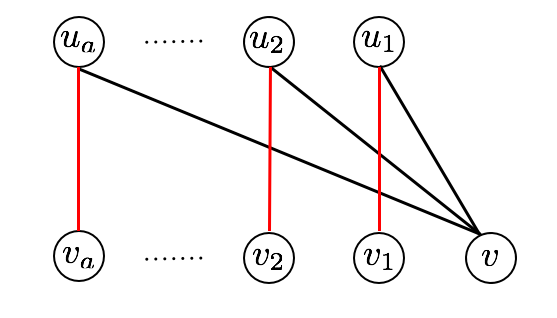
\includegraphics[width=.39\textwidth]{images/greedy.png}
\caption{This diagram shows one step of the greedy algorithm. When $v$ selects edges to $u_1,\ldots, u_a$, it potentially removes $v_1,\ldots, v_a$ from the pool of candidates that are available. The potentially invalidated edges are shown in red.}
\end{figure}

This approximation guarantee is as good as we can expect,
since for $a=1$ we recover the familiar $1/2$-approximation
of the greedy algorithm for matchings. Furthermore, even in the case of matchings ($a=1$),
randomizing the order in which the vertices are processed is still
known to leave a constant factor gap in the quality of the solution
~\cite{KarpVaziraniVazirani1990}. Despite this result, the greedy
algorithm fares much better when we analyze its expected performance.
Switching to the
{\bf Erd\"{o}s-Renyi model}~\cite{ErdosRenyi59} instead of the fixed degree model used in
the previous section, we now prove the near optimality of the
greedy algorithm for the $(c, a)$-recommendation subgraph problem.
Recall that in this model (sometimes referred to as $G_{n,p}$), each possible edge is inserted with probability $p$ independent of other edges. In our version $G_{l,r,p}$, we only add edges from $L$ to $R$ each with probability $p$ independent of other edges in this complete bipartite candidate graph.  For technical reasons, we need to assume that $lp \geq 1$ in the following theorem. However, this is a very weak assumption since $lp$ is simply the expected degree of a vertex $v\in L$. Typical values for $p$ for our applications will be $\Omega(\log(l)/l)$ making the expected degree $lp=\Omega(\log l)$.

\begin{thm}
Let $G=(L,R,E)$ be a graph drawn from the $G_{l,r,p}$ where $lp \geq 1$. If $S$ is the size of the $(c,a)$-recommendation subgraph produced by the greedy algorithm, then:
\[ \emph{\E}[S] \geq r - \frac{a(lp)^{a-1}}{(1-p)^a} \sum_{i=0}^{r-1}(1-p)^{l-\frac{ia}{c}}\]
\end{thm}
\begin{proof}
Note that if edges are generated uniformly, we can consider the
graph as being revealed to us one vertex at a time as the greedy
algorithm runs. In particular, consider the event $X_{i+1}$ that the
greedy algorithm matches the $(i+1)^{st}$ vertex it inspects. While,
$X_{i+1}$ is dependent on $X_1,\ldots, X_i$, the worst condition for
$X_{i+1}$ is when all the previous $i$ vertices were from the same
vertices in $L$, which are now not available for matching the
$(i+1)^{st}$ vertex. The maximum number of such invalidated vertices
is at most $\lceil ia/c \rceil$. Therefore, the bad event
is that we have fewer than $a$ of the at least $l-\lceil ia/c \rceil$ 
available vertices having an edge to this vertex. The probability of this
bad event is at most $\Pr[Y\sim Bin(l-\frac{ia}{c},p): Y < a]$, the
probability that a Binomial random variable with $l - \frac{ia}{c}$
trials of probability $p$ of success for each trial has less than $a$
successes. We can bound this probability by using a union bound and
upper-bounding $\Pr[Y\sim Bin(l-\frac{ia}{c},p): Y = t]$ for each 
$0 \leq t \leq a-1$. By using the trivial estimate that
$\binom{n}{i} \leq n^i$ for all $n$ and $i$, we obtain:

\begin{align*}
      \Pr[Y\sim Bin(l-\frac{ia}{c},p): Y = t]
&=    \binom{l-\frac{ia}{c}}{t} (1-p)^{l-\frac{ia}{c}-t}p^{t} \\
&\leq \left(l-\frac{ia}{c}\right)^t (1-p)^{l-\frac{ia}{c}-t} p^{t} \\
&\leq (lp)^t (1-p)^{l-\frac{ia}{c}-t} 
\end{align*}

Notice that the largest exponent $lp$ can take within the bounds of
our sum is $a-1$. Similarly, the smallest exponent $(1-p)$ can take
within the bounds of our sum is $l-\frac{ia}{c}-a+1$. Now applying
the union bound gives:

\begin{align*}
&           \Pr[Y\sim Bin(l-\frac{ia}{c},p): Y < a] \\
&\leq  \sum_{t=0}^{a-1} \Pr[Y\sim Bin(l-\frac{ia}{c},p): Y = t] \\
&\leq  \sum_{t=0}^{a-1} (lp)^t (1-p)^{l-\frac{ia}{c}-t} \\
&=     a(lp)^{a-1} (1-p)^{l-\frac{ia}{c}-a+1}
\end{align*}

Finally, summing over all the $X_i$ using the linearity of
expectation and this upper bound, we obtain

\begin{align*}
      \E[S]
&\geq r - \sum_{i=0}^{r-1} \E[\lnot X_i] \\
&\geq r - \sum_{i=0}^{r-1} \Pr[Y \sim Bin(l-\frac{ia}{c},p): Y < a] \\
&\geq r - a(lp)^{a-1}\sum_{i=0}^{r-1}(1-p)^{l-\frac{ia}{c}-a+1}
\end{align*}
\end{proof}

Asymptotically, this result explains why the greedy
algorithm does much better in expectation than $1/(a+1)$ guarantee we
can prove in the worst case.
%Arda: The following does not make much sense to me either. I assume you are talking about lc >> ra to get high coverage from the left to the right, but I dont see how you get the expressions that are sublinear in l??
In particular, suppose $a$ and $c$ are fixed and that
$l/r$ is taken to be a constant as both $l$ and $r$ tend to $\infty$. In the realm where sublinear error is possible (i.e. when $lc/a>r$) each term in the sum above becomes $\Theta(l^{-\epsilon})$ for some $\epsilon>0$ if we set $p=\Theta(\log(l)/l)$. Consequently, the error term reduces to $\Theta(l^{1-\epsilon}\log^a(l))$ which is sublinear on the number of vertices.
